\documentclass[12pt,]{article}
\usepackage{lmodern}
\usepackage{amssymb,amsmath}
\usepackage{ifxetex,ifluatex}
\usepackage{fixltx2e} % provides \textsubscript
\ifnum 0\ifxetex 1\fi\ifluatex 1\fi=0 % if pdftex
  \usepackage[T1]{fontenc}
  \usepackage[utf8]{inputenc}
\else % if luatex or xelatex
  \ifxetex
    \usepackage{mathspec}
  \else
    \usepackage{fontspec}
  \fi
  \defaultfontfeatures{Ligatures=TeX,Scale=MatchLowercase}
\fi
% use upquote if available, for straight quotes in verbatim environments
\IfFileExists{upquote.sty}{\usepackage{upquote}}{}
% use microtype if available
\IfFileExists{microtype.sty}{%
\usepackage{microtype}
\UseMicrotypeSet[protrusion]{basicmath} % disable protrusion for tt fonts
}{}
\usepackage[left=1in, right=1in, top=1in, bottom=1in, headheight=12pt, letterpaper]{geometry}
\usepackage{hyperref}
\hypersetup{unicode=true,
            pdftitle={Quantifying and partitioning uncertainty to improve ecological forecasts},
            pdfauthor={Andrew T. Tredennick\^{}\{1\}, Peter B. Adler\^{}1, and others\^{}\{2\}},
            pdfborder={0 0 0},
            breaklinks=true}
\urlstyle{same}  % don't use monospace font for urls
\usepackage{graphicx,grffile}
\makeatletter
\def\maxwidth{\ifdim\Gin@nat@width>\linewidth\linewidth\else\Gin@nat@width\fi}
\def\maxheight{\ifdim\Gin@nat@height>\textheight\textheight\else\Gin@nat@height\fi}
\makeatother
% Scale images if necessary, so that they will not overflow the page
% margins by default, and it is still possible to overwrite the defaults
% using explicit options in \includegraphics[width, height, ...]{}
\setkeys{Gin}{width=\maxwidth,height=\maxheight,keepaspectratio}
\IfFileExists{parskip.sty}{%
\usepackage{parskip}
}{% else
\setlength{\parindent}{0pt}
\setlength{\parskip}{6pt plus 2pt minus 1pt}
}
\setlength{\emergencystretch}{3em}  % prevent overfull lines
\providecommand{\tightlist}{%
  \setlength{\itemsep}{0pt}\setlength{\parskip}{0pt}}
\setcounter{secnumdepth}{0}
% Redefines (sub)paragraphs to behave more like sections
\ifx\paragraph\undefined\else
\let\oldparagraph\paragraph
\renewcommand{\paragraph}[1]{\oldparagraph{#1}\mbox{}}
\fi
\ifx\subparagraph\undefined\else
\let\oldsubparagraph\subparagraph
\renewcommand{\subparagraph}[1]{\oldsubparagraph{#1}\mbox{}}
\fi

%%% Use protect on footnotes to avoid problems with footnotes in titles
\let\rmarkdownfootnote\footnote%
\def\footnote{\protect\rmarkdownfootnote}

%%% Change title format to be more compact
\usepackage{titling}

% Create subtitle command for use in maketitle
\newcommand{\subtitle}[1]{
  \posttitle{
    \begin{center}\large#1\end{center}
    }
}

\setlength{\droptitle}{-2em}
  \title{Quantifying and partitioning uncertainty to improve ecological forecasts}
  \pretitle{\vspace{\droptitle}\centering\huge}
  \posttitle{\par}
  \author{Andrew T. Tredennick\(^{1}\), Peter B. Adler\(^1\), and others\(^{2}\)}
  \preauthor{\centering\large\emph}
  \postauthor{\par}
  \date{}
  \predate{}\postdate{}

\usepackage{mathptmx}
\usepackage{upgreek}
\usepackage{bm}
\usepackage{setspace}
\usepackage{booktabs}
\doublespacing
\usepackage{lineno}
\linenumbers

\begin{document}
\maketitle

\setlength{\abovedisplayskip}{0pt} \raggedright

\(^1\) Department of Wildland Resources and the Ecology Center, Utah
State University, Logan, UT, United States

\(^2\) Department of somewhere

\section{Abstract}\label{abstract}

Making informed ecosystem management decisions in the face of rapid
environmental change requires forecasts from models of ecological
processes. However, forecasts from ecological models are often
associated with high degrees of uncertainty, making it difficult for
such forecasts to inform decision-making processes. To make progress
toward the goal of reliable and informative ecological forecasts, we
need to know from where forecast uncertainty arises. Such knowledge can
guide investment in future research that will most improve forecast
skill. Here we develop a simulation-based approach for quantifying and
partitioning forecast uncertainty from Bayesian state-space models that
overcomes the limitations of previous analytical approaches. Our
approach is similar to an Analysis of Variance, where the total variance
of a forecast is paritioned among its constituent parts, namely initial
conditions uncertainty, parameter uncertainty, driver uncertainty,
process error, and their interactions. We demonstrate the approach with
simulated data and with an empirical example using data from the
Yellowstone bison herd. We also provide general functions written in the
statistical programming language R, which should allow others using
Bayesian state-space models to employ our approach in their own
research.

\emph{Keywords: forecast, Markov chain Monte Carlo, prediction,
population model, uncertainty}

\section{Introduction}\label{introduction}

A fundamental challenge facing society is to predict the ecological
impacts of global environmental changes such as nitrogen deposition,
climate change, and habitat fragmentation. Each of these global change
drivers have now exceeded their historical ranges of variability
(Steffen et al. 2015), ushering in a no-analog era in which the past
cannot predict the future. We can, however, look to the past to
parameterize models that allow us to forecast the future states of
ecological systems (Clark et al. 2001, Dietze et al. 2018). Ecologists
are in an excellent position to meet this forecasting challenge because
we have spent decades gaining understanding of the processes that
regulate populations, communities, and ecosystems. However, we lack a
systematic understanding of the current limits to ecological forecasts.
As a result, we do not know how to allocate research effort to improve
our forecasts.

Making poor forecasts is inevitable as ecology matures into a more
predictive science. The key is to learn from our failures so that
forecasts become more accurate over time. The success of meteorological
forecasting tells us that basic research on the causes of forecast
uncertainty is an essential component of this learning process (Bauer et
al. 2015).

Various approaches have been used to characterize and partition forecast
uncertainty (Sobol' 1993, Cariboni et al. 2007). For example, consider a
dynamic model designed to predict some state \emph{y} in the future
(\(y_{t+1}\)) based on the current state (\(y_{t}\)), an environmental
driver(s) (\(x\)), parameters (\(\theta\)), and process error
(\(\epsilon\)). We can then write a general form of the model as:

\begin{align}
y_{t+1} = f(y_t, x_t|\theta) + \epsilon_{t+1},
\end{align}

which states that \(y\) at time \(t+1\) is a function of \(y\) and \(x\)
at time \(t\) conditional on the model parameters (\(\theta\)) plus
process error (\(\epsilon\)). Ignoring covariance among factors, Dietze
(2017), following Sobol' (1993) and Cariboni et al. (2007), suggests
that forecast variance (\(Var[y_{t+1}]\)) is approximately:

\begin{align}
Var[y_{t+1}] \approx \underbrace{\left(\frac{\delta f}{\delta y} \right)^2}_{\text{stability}} 
               \underbrace{\vphantom{ \left(\frac{\delta f}{\delta y} \right)^2 } Var[y_t]}_{\text{IC uncert.}} +
               \underbrace{\vphantom{ \left(\frac{\delta f}{\delta y} \right)^2 }\left(\frac{\delta f}{\delta x} \right)^2}_{\text{driver sens.}} 
               \underbrace{\vphantom{ \left(\frac{\delta f}{\delta y} \right)^2 } Var[x_t]}_{\text{driver uncert.}} +
               \underbrace{\vphantom{ \left(\frac{\delta f}{\delta y} \right)^2 }\left(\frac{\delta f}{\delta \theta} \right)^2}_{\text{param sens.}}
               \underbrace{\vphantom{ \left(\frac{\delta f}{\delta y} \right)^2 } Var[\theta]}_{\text{param. uncert.}} +
               \underbrace{\vphantom{ \left(\frac{\delta f}{\delta y} \right)^2 } Var[\epsilon_{t+1}]}_{\text{process error}},
\end{align}

where each additive term follows a pattern of \emph{sensitivity} times
\emph{variance} and ``IC uncert.'' refers to ``\emph{I}nitial
\emph{C}onditions uncertainty.'' The variance attributable to any
particular factor is a function of how sensitive the model is to the
factor and the variance of that factor. For example, the atmosphere is a
chaotic system, meaning its dynamics are internally unstable and
sensitive to initial conditions uncertainty. This is why billions of
dollars are spent each year to measure meterological variables --
meterologists learned that the key to reducing forecast error
\((Var[y_{t+1}])\) was to reduce the uncertainty of initial conditions
(\(Var[y_t]\)).

In contrast, ecologists are attempting to make actionable forecasts with
little knowledge of which term in Eq. 2 dominates forecast error.
Knowing which term dominates forecast error in different ecological
settings will advance our fundamental understanding of the natural world
and immediately impact practical efforts to monitor, model, and predict
ecological dynamics.

\section{A simulation-based approach for partitioning
uncertainty}\label{a-simulation-based-approach-for-partitioning-uncertainty}

Analytical expressions of forecast uncertainty must rely on simplifying
assumptions. Two important assumptions are (1) that different sources of
uncertainty do not interact and (2) that the system of equations is
linear. These analytical expressions are important for guiding our
intuition, but these strict assumptions limit our ability to partition
forecast uncertainty in practice. Thus, we present a simulation approach
that is entirely model-based and requires no assumptions, other than
those embedded in the model itself. We are building on the ideas put
forth by Dietze (2017), who suggested a simulation approach for
quantifying the terms in Eq. 2. Here we test the general idea using
simulated data and extend the approach to consider interactions among
sources of uncertainty.

As a starting point, consider the general state-space model

\begin{gather}
\left[y_{(t)} \;|\; z_{(t)}, \sigma^2_{\text{o}}\right], \\
\left[z_{(t)} \;|\; \mu_{(t)}, \sigma^2_{\text{p}}\right], \\
\mu_{(t)} = g \left(z_{(t-1)},\textbf{x}'_{(t)}, \bm{\uptheta} \right),
\end{gather}

\noindent{}where \(y_{(t)}\) is the observed state at time \emph{t},
\(z_{(t)}\) is the latent state at time \emph{t}, \(\mu_{(t)}\) is the
determinstic prediction of \emph{z} at time \emph{t} from the process
model \emph{g}, which is a function of \emph{z} at time \emph{t-1}, a
vector of covariates at time \emph{t}, and a set of unknown parameters,
\(\bm{\uptheta}\). \(\sigma^2_{\text{o}}\) is observation error and
\(\sigma^2_{\text{p}}\) is process error. The notation
\(\left[a \;|\; b, c\right]\) reads, ``the probability of \emph{a} given
\emph{b} and \emph{c}.''

This type of model is easily fit using Bayesian methods and Markov chain
Monte carlo (MCMC) algorithms. The posterior distribution of all
unkowns, including states and parameters, is estimated over \emph{K}
MCMC iterations.

\begin{figure}
\centering
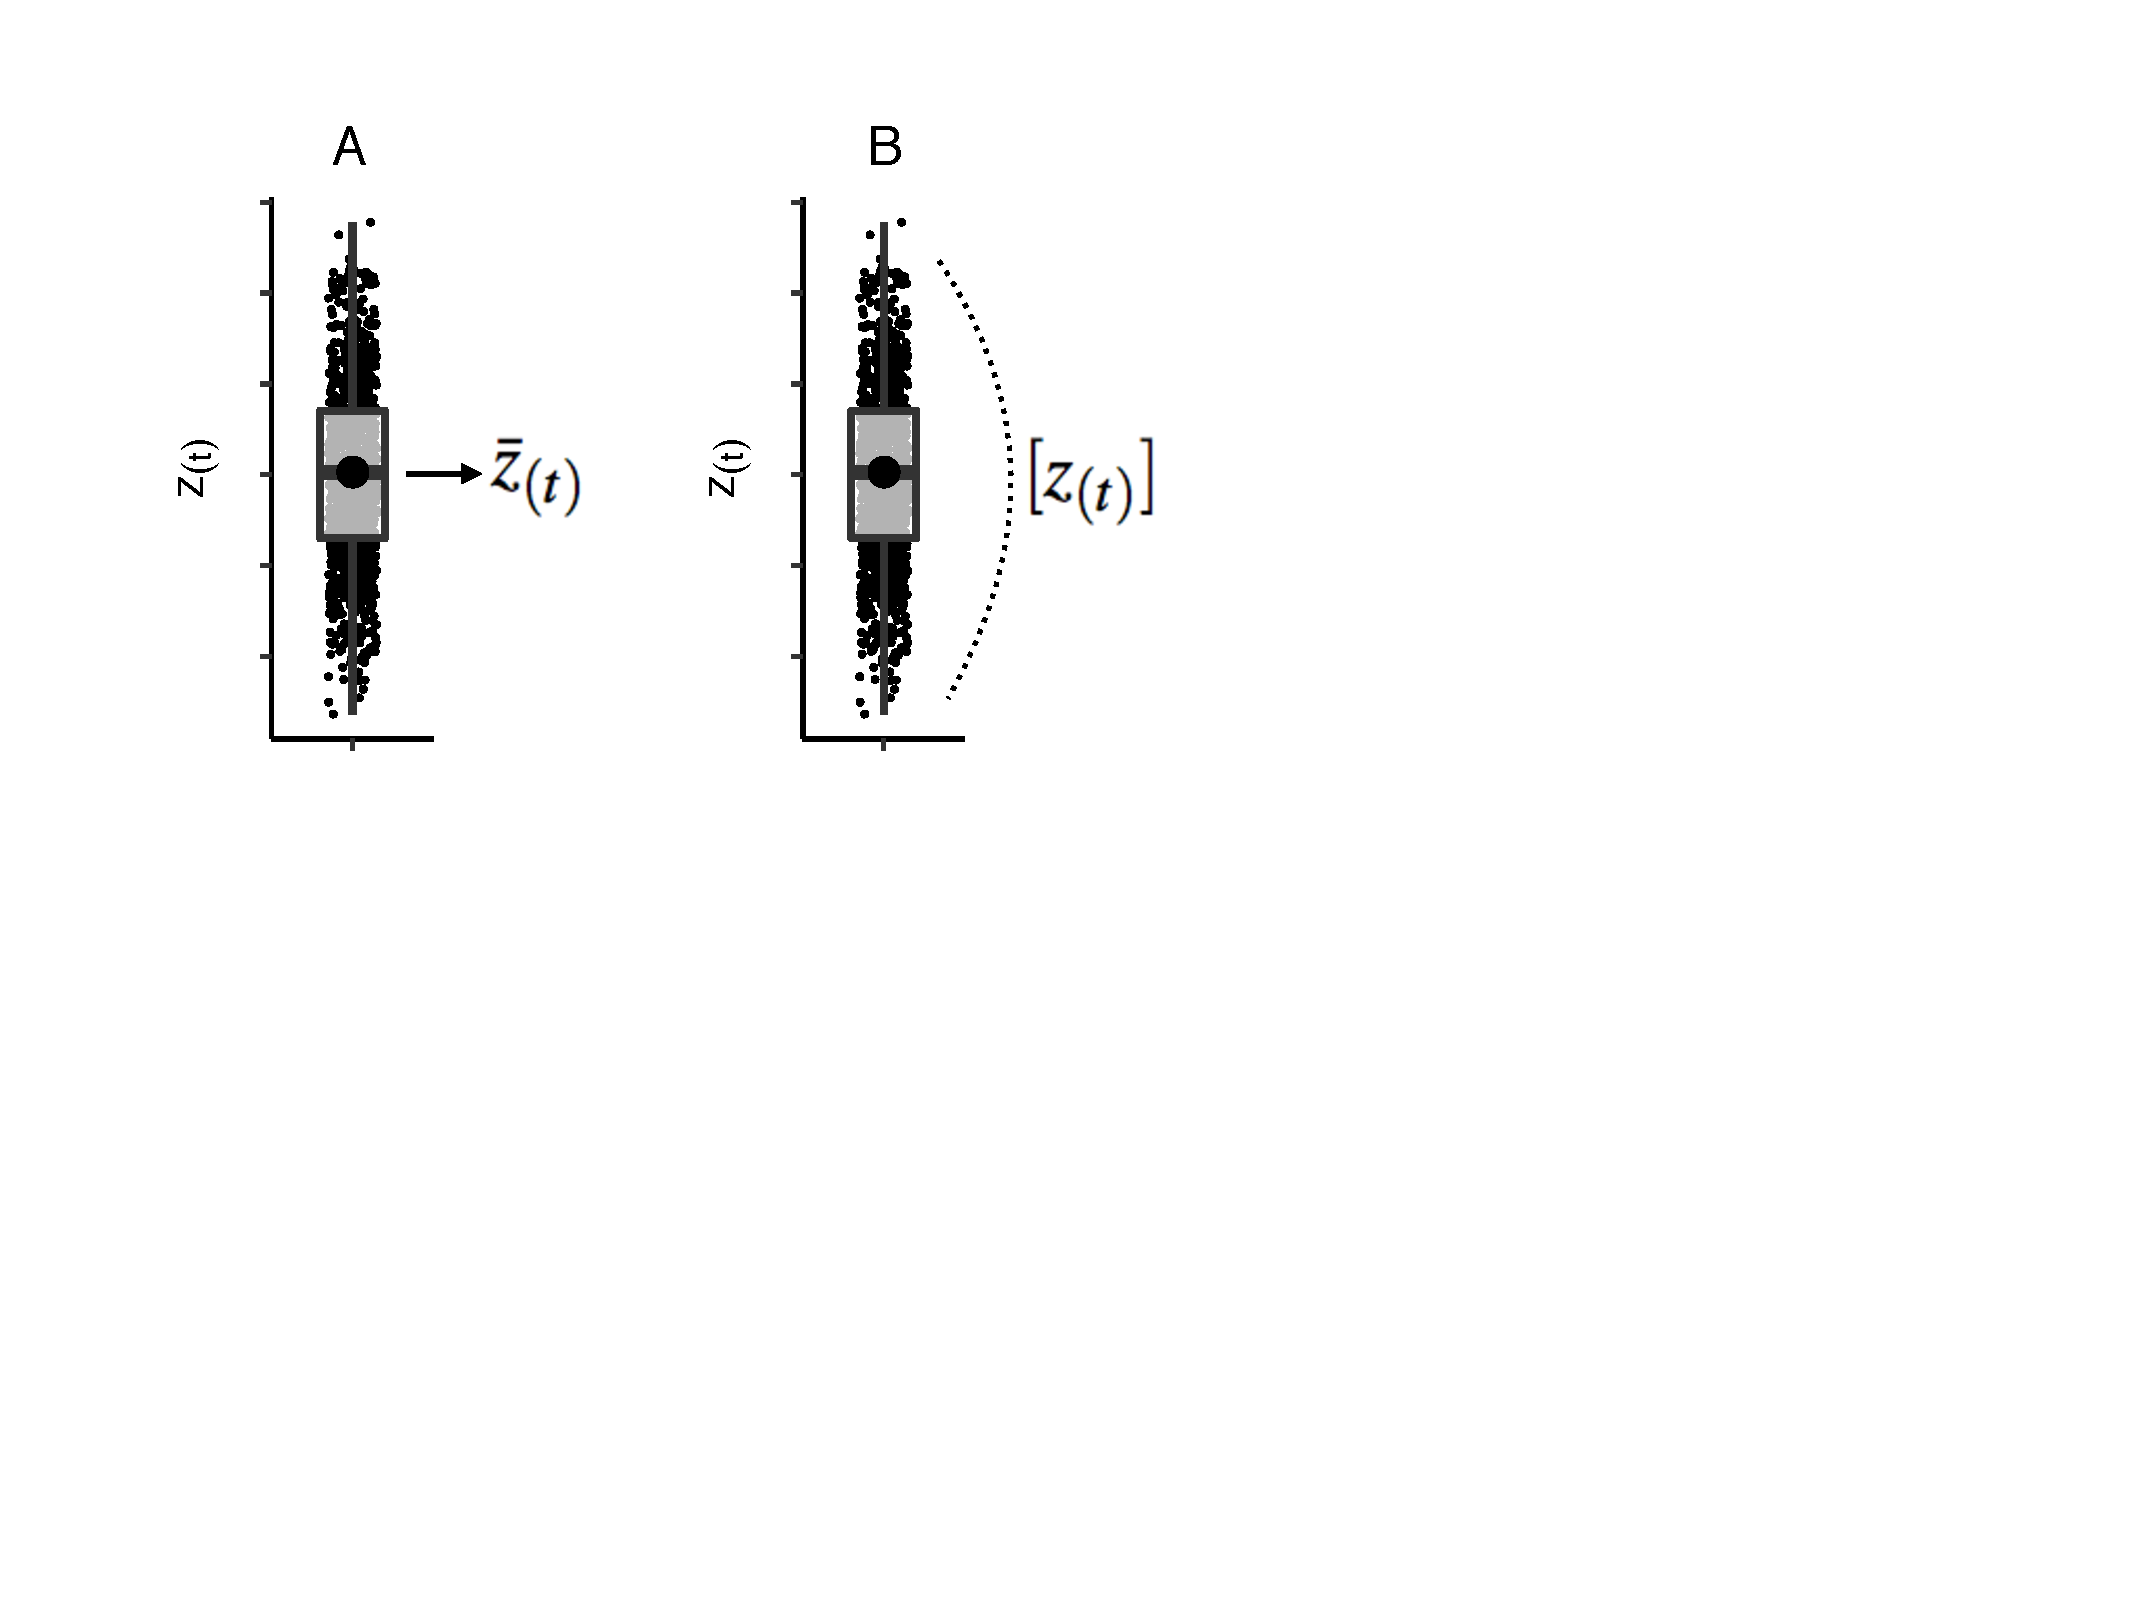
\includegraphics[height=2.00000in]{../figures/init_cond_example.pdf}
\caption{Example.}
\end{figure}

\section*{References}\label{references}
\addcontentsline{toc}{section}{References}

\hypertarget{refs}{}
\hypertarget{ref-Bauer2015}{}
Bauer, P., A. Thorpe, and G. Brunet. 2015. The quiet revolution of
numerical weather prediction. Nature 525:47--55.

\hypertarget{ref-Cariboni2007}{}
Cariboni, J., D. Gatelli, R. Liska, and A. Saltelli. 2007. The role of
sensitivity analysis in ecological modelling. Ecological Modelling
203:167--182.

\hypertarget{ref-Clark2001}{}
Clark, J. S., S. R. Carpenter, M. Barber, S. Collins, A. Dobson, J. A.
Foley, D. M. Lodge, M. Pascual, R. Pielke, W. Pizer, C. Pringle, W. V.
Reid, K. A. Rose, O. Sala, W. H. Schlesinger, D. H. Wall, and D. Wear.
2001. Ecological forecasts: an emerging imperative. Science
293:657--660.

\hypertarget{ref-Dietze2017a}{}
Dietze, M. C. 2017. Prediction in ecology: A first-principles framework.
Ecological Applications 27:2048--2060.

\hypertarget{ref-Dietze2018}{}
Dietze, M. C., A. Fox, L. M. Beck-Johnson, J. L. Betancourt, M. B.
Hooten, C. S. Jarnevich, T. H. Keitt, M. A. Kenney, C. M. Laney, L. G.
Larsen, H. W. Loescher, C. K. Lunch, B. C. Pijanowski, J. T. Randerson,
E. K. Read, A. T. Tredennick, R. Vargas, K. C. Weathers, and E. P.
White. 2018. Iterative near-term ecological forecasting: Needs,
opportunities, and challenges. Proceedings of the National Academy of
Sciences 115:1424--1432.

\hypertarget{ref-Sobol1993}{}
Sobol', I. 1993. Sensitivity Estimates for Nonlinear Mathematical
Models.

\hypertarget{ref-Steffen2015}{}
Steffen, W., K. Richardson, J. Rockström, S. Cornell, I. Fetzer, E.
Bennett, R. Biggs, and S. Carpenter. 2015. Planetary boundaries: Guiding
human development on a changing planet. Science 348:1217.


\end{document}
